\section{Experimental Setup and Results}

\subsection{Experimental Setup}
This section follows the experimental configuration consolidated by Trần Đặng Hiển Long and uses it as the authoritative setup for the final report. The study evaluates three tokenization strategies---word-level, character-level, and BPE---on four benchmark corpora.

\subsubsection{Preprocessing Pipeline}
\begin{figure}[H]
    \centering
    \begin{tikzpicture}[node distance=1.5cm, every node/.style={fill=white, font=\footnotesize}, align=center]
        \node (raw) [draw, rectangle] {Raw Text \\ (e.g., WikiText-103)};
        \node (norm) [draw, rectangle, below of=raw] {Normalization \\ (Lowercasing, Smart Quotes $\rightarrow$ ASCII)};
        \node (clean) [draw, rectangle, below of=norm] {Character Filtering \\ (Regex Policy)};
        \node (chunk) [draw, rectangle, below of=clean] {Chunking \\ (Text8: 200w / Enwik8: 1000ch)};
        \node (token) [draw, diamond, aspect=2, below of=chunk, node distance=2cm] {Tokenization Type?};
        
        \draw [->] (raw) -- (norm);
        \draw [->] (norm) -- (clean);
        \draw [->] (clean) -- (chunk);
        \draw [->] (chunk) -- (token);
        
        \node (word) [draw, rectangle, below left of=token, node distance=2.5cm, xshift=-1cm] {Word-level};
        \node (char) [draw, rectangle, below of=token, node distance=2.5cm] {Character-level};
        \node (bpe) [draw, rectangle, below right of=token, node distance=2.5cm, xshift=1cm] {BPE (Subword)};
        
        \draw [->] (token) -| (word);
        \draw [->] (token) -- (char);
        \draw [->] (token) -| (bpe);
    \end{tikzpicture}
    \caption{Preprocessing and Tokenization Flowchart}
    \label{fig:pipeline_flow}
\end{figure}

The preprocessing pipeline uses a fixed random seed of 42. Before tokenization, text is lowercased, tabs and line breaks are normalized, and repeated whitespace is collapsed. A strict character-filtering regular expression is applied to keep only alphanumeric symbols, spaces, and a selected punctuation subset: \texttt{[a-z0-9\textbackslash s\textbackslash .\textbackslash ,!\textbackslash ?;:'"\textbackslash -\textbackslash (\textbackslash )]}.

\subsubsection{Datasets and Chunking}
Existing train/validation/test splits are reused for \textit{One Billion Word} and \textit{WikiText-103}. For \textit{Text8} and \textit{Enwik8}, the data is shuffled and split into 90\% train, 5\% validation, and 5\% test. To manage sequence geometry during training, \textit{Text8} is chunked into 200-word segments, while \textit{Enwik8} uses segments of 1000 characters.

\subsubsection{Tokenizer Configuration}
All tokenizers share the special tokens \texttt{<PAD>}, \texttt{<UNK>}, \texttt{<BOS>}, and \texttt{<EOS>}.
\begin{itemize}
    \item \textbf{Word-level:} Regex-based segmentation with a target vocabulary sweep.
    \item \textbf{Character-level:} Character-set vocabulary derived from the training corpus.
    \item \textbf{BPE:} Implemented via the Hugging Face \texttt{tokenizers} library with a \texttt{Whitespace()} pre-tokenizer.
\end{itemize}

\subsubsection{Language Modeling Configuration}
To examine downstream effects, we train an LSTM-based language model with the following shared hyperparameters: embedding size 128, hidden size 256, 2 layers, batch size 32, sequence length 128, learning rate 0.001, and random seed 42. Perplexity and avg. epoch time are calculated across a fixed budget of 3--5 epochs depending on the comparison.

\subsection{Tokenization Evaluation}
The performance metrics for each tokenizer are summarized across multiple configurations. The data reveals a clear inverse relationship between the vocabulary size and the resulting average sequence length ($L_{avg}$), alongside the critical trade-off with the Out-of-Vocabulary (OOV) rate.

\begin{table}[h]
\centering
\caption{Consolidated Benchmarks: OOV Penalties vs. Optimized Subword Compression}
\label{tab:final_relative_results}
\resizebox{\textwidth}{!}{
\begin{tabular}{|l|l|r|l|r|l|}
\hline
\textbf{Dataset} & \textbf{Tokenizer} & \textbf{Vocab} & \textbf{Avg. Seq. Len} $\downarrow$ & \textbf{OOV (\%)} $\uparrow$ & \textbf{Comp. Ratio} $\downarrow$ \\ \hline
\multirow{7}{*}{\textbf{Text8}} & Char & 31 & 1178.08 (+489.0\%) & 0.00\% & 1.00 (+489.0\%) \\ \cline{2-6}
 & BPE-2k & 2,000 & 318.36 (+59.2\%) & 0.00\% & 0.27 (+59.2\%) \\ \cline{2-6}
 & BPE-8k & 8,000 & 247.50 (+23.8\%) & 0.00\% & 0.21 (+23.8\%) \\ \cline{2-6}
 & BPE-16k & 16,000 & 226.54 (+13.3\%) & 0.00\% & 0.19 (+13.3\%) \\ \cline{2-6}
 & BPE-32k & 32,000 & 213.80 (+6.9\%) & 0.00\% & 0.18 (+6.9\%) \\ \cline{2-6}
 & BPE-50k & 50,000 & 208.95 \underline{\textbf{(+4.5\%)}} & 0.00\% & 0.18 \underline{\textbf{(+4.5\%)}} \\ \cline{2-6}
 & Word & 50,000 & \textbf{200.00} & \textbf{2.77\%} & \textbf{0.17} \\ \hline \hline
\multirow{7}{*}{\textbf{Wiki-103}} & Char & 52 & 431.72 (+421.3\%) & 0.00\% & 1.00 (+421.3\%) \\ \cline{2-6}
 & BPE-2k & 2,000 & 125.78 (+51.9\%) & 0.00\% & 0.29 (+51.9\%) \\ \cline{2-6}
 & BPE-8k & 8,000 & 99.86 (+20.6\%) & 0.00\% & 0.23 (+20.6\%) \\ \cline{2-6}
 & BPE-16k & 16,000 & 92.65 (+11.9\%) & 0.00\% & 0.21 (+11.9\%) \\ \cline{2-6}
 & BPE-32k & 32,000 & 88.53 (+6.9\%) & 0.00\% & 0.21 (+6.9\%) \\ \cline{2-6}
 & BPE-50k & 50,000 & 86.82 \underline{\textbf{(+4.8\%)}} & 0.00\% & 0.20 \underline{\textbf{(+4.8\%)}} \\ \cline{2-6}
 & Word & 45,379 & \textbf{82.82} & \textbf{3.42\%} & \textbf{0.19} \\ \hline \hline
\multirow{7}{*}{\textbf{One Billion}} & Char & 52 & 135.27 (+408.2\%) & 0.00\% & 1.00 (+408.2\%) \\ \cline{2-6}
 & BPE-2k & 2,000 & 39.08 (+46.8\%) & 0.00\% & 0.29 (+46.8\%) \\ \cline{2-6}
 & BPE-8k & 8,000 & 30.95 (+16.3\%) & 0.00\% & 0.23 (+16.3\%) \\ \cline{2-6}
 & BPE-16k & 16,000 & 28.98 (+8.9\%) & 0.00\% & 0.21 (+8.9\%) \\ \cline{2-6}
 & BPE-32k & 32,000 & 28.03 (+5.3\%) & 0.00\% & 0.21 (+5.3\%) \\ \cline{2-6}
 & BPE-50k & 38,379 & 27.83 \underline{\textbf{(+4.5\%)}} & 0.00\% & 0.21 \underline{\textbf{(+4.5\%)}} \\ \cline{2-6}
 & Word & 29,164 & \textbf{26.62} & \textbf{3.83\%} & \textbf{0.20} \\ \hline \hline
\multirow{7}{*}{\textbf{Enwik8}} & Char & 52 & 925.72 (+377.2\%) & 0.00\% & 1.00 (+377.2\%) \\ \cline{2-6}
 & BPE-2k & 2,000 & 290.28 (+49.6\%) & 0.00\% & 0.31 (+49.6\%) \\ \cline{2-6}
 & BPE-8k & 8,000 & 231.30 (+19.2\%) & 0.00\% & 0.25 (+19.2\%) \\ \cline{2-6}
 & BPE-16k & 16,000 & 213.33 (+10.0\%) & 0.00\% & 0.23 (+10.0\%) \\ \cline{2-6}
 & BPE-32k & 32,000 & 201.98 (+4.1\%) & 0.00\% & 0.22 (+4.1\%) \\ \cline{2-6}
 & BPE-50k & 50,000 & 197.24 \underline{\textbf{(+1.7\%)}} & 0.00\% & 0.218 \underline{\textbf{(+2.2\%)}} \\ \cline{2-6}
 & Word & 50,000 & \textbf{194.00} & \textbf{3.41\%} & \textbf{0.213} \\ \hline
\end{tabular}
}
\end{table}

Our results confirm that BPE effectively serves as a "sweet spot" in the tokenization landscape. Although Word-level tokenization provides the theoretical baseline for compression (highlighted in \textbf{bold} in Table~\ref{tab:final_relative_results}), it consistently fails due to high OOV rates.

\subsubsection{Detailed Word-level Tokenization Results}
To investigate the vocabulary bottleneck, we evaluated word-level tokenization across three vocabulary scales (5,000, 10,000, and 50,000 tokens).

\begin{table}[H]
\centering
\caption{Word-level Tokenization Results (Scaling Effects)}
\renewcommand{\arraystretch}{1.1}
\begin{tabular}{|l|c|c|c|c|c|}
\hline
\textbf{Vocab Size} & \textbf{Split} & \textbf{Enwik8} & \textbf{One Billion} & \textbf{Text8} & \textbf{WikiText-103} \\ \hline
\multirow{2}{*}{5,000} & OOV (\%) & 15.55 & 11.72 & 16.18 & 14.84 \\ \cline{2-6}
& Comp. Ratio & 0.209 & 0.196 & 0.170 & 0.189 \\ \hline
\multirow{2}{*}{10,000} & OOV (\%) & 10.43 & 6.85 & 10.37 & 9.65 \\ \cline{2-6}
& Comp. Ratio & 0.209 & 0.196 & 0.169 & 0.189 \\ \hline
\multirow{2}{*}{50,000} & OOV (\%) & \textbf{3.41} & \textbf{1.31} & \textbf{2.77} & \textbf{2.76} \\ \cline{2-6}
& Comp. Ratio & 0.209 & 0.196 & 0.169 & 0.189 \\ \hline
\end{tabular}
\end{table}

\textbf{Insights from Word-level Sweeps:}
\begin{itemize}
    \item \textbf{Vocab 5k:} A 5,000-word limit causes severe semantic loss, with OOV rates spiking to $\sim$16\% on Text8 and Enwik8.
    \item \textbf{Vocab 10k:} Doubling the vocabulary size roughly halves the OOV rate on the One Billion Word dataset, yet $\sim$10\% OOV on other benchmarks remains problematic.
    \item \textbf{Vocab 50k:} At 50,000 tokens, the tokenizer achieves acceptable semantic retention (OOV $\le$ 3.4\%) and maintains high compression efficiency (0.16--0.20), though it still cannot reach the 0\% OOV threshold required for total robustness.
\end{itemize}

\subsubsection{Character-level Tokenization Results}
Character-level tokenization treats every individual character as a distinct token, completely eliminating OOV at the cost of extreme sequence inflation.

\begin{table}[H]
\centering
\caption{Character-level Tokenization Results}
\renewcommand{\arraystretch}{1.1}
\begin{tabular}{|l|c|c|c|c|}
\hline
\textbf{Metric (Test Split)} & \textbf{Enwik8} & \textbf{One Billion} & \textbf{Text8} & \textbf{WikiText-103} \\ \hline
\textbf{Absolute Vocab Size} & \textbf{52} & \textbf{52} & \textbf{31} & \textbf{52} \\ \hline
Avg Seq Length & 925.72 & 135.27 & 1178.08 & 431.72 \\ \hline
OOV Rate (\%) & 0 & 0 & 0 & 0 \\ \hline
Compression Ratio & 1.000 & 1.000 & 1.000 & 1.000 \\ \hline
\end{tabular}
\end{table}

\textbf{Insights from Character-level Trials:}
\begin{itemize}
    \item \textbf{Microscopic Vocabulary:} Uses only 31--52 tokens, drastically reducing the embedding memory footprint.
    \item \textbf{Sequence Inflation:} Sequence lengths explode (e.g., $\sim$1178 on Text8), placing an immense computational burden on recurrent models and hindering long-term context capture.
\end{itemize}

\subsubsection{BPE Results and Vocabulary Scaling}
BPE serves as the optimal bridge, providing complete OOV elimination while maintaining compression ratios near those of word-level models.

\begin{figure}[H]
    \centering
    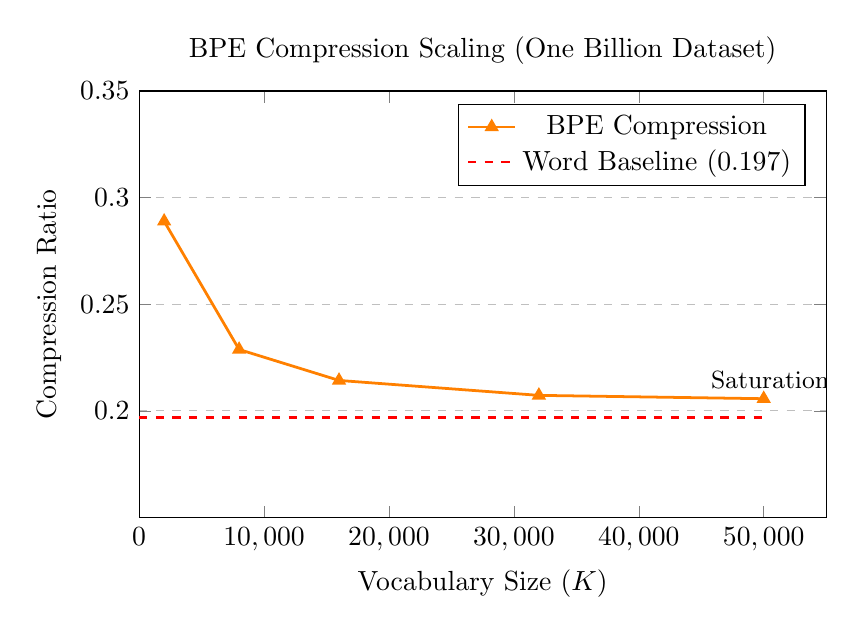
\begin{tikzpicture}
    \begin{axis}[
        title={BPE Compression Scaling (One Billion Dataset)},
        xlabel={Vocabulary Size ($K$)},
        ylabel={Compression Ratio},
        xmin=0, xmax=55000,
        ymin=0.15, ymax=0.35, 
        xtick={0, 10000, 20000, 30000, 40000, 50000},
        ytick={0, 0.20, 0.25, 0.30, 0.35},
        scaled x ticks=false,
        xticklabel style={
            /pgf/number format/fixed,
            /pgf/number format/1000 sep={,}
        },
        % ------------------------------------------
        legend pos=north east,
        ymajorgrids=true,
        grid style=dashed,
        width=0.85\textwidth,
        height=7cm,
    ]

    % BPE Compression Curve
    \addplot[
        color=orange,
        mark=triangle*,
        line width=1pt,
        ]
        coordinates {
        (2000, 0.2889)(8000, 0.2288)(16000, 0.2143)(32000, 0.2073)(50000, 0.20573)
        };
        \addlegendentry{BPE Compression}

    % Word-level Baseline Ratio
    \addplot[
        color=red,
        dashed,
        line width=1pt,
        domain=0:50000,
    ] {0.1968};
    \addlegendentry{Word Baseline (0.197)}

    % Saturation Point Label
    \node[anchor=south west] at (axis cs:45000, 0.20573) {\small Saturation};

    \end{axis}
    \end{tikzpicture}
    \caption{BPE Compression Ratio correlation with K = 2k, 4k, 8k, 16k, 32k, 50k. The graph illustrates how BPE approaches the theoretical maximum density of Word-level tokenization without the cost of OOV errors.}
    \label{fig:compression_one_billion}
\end{figure}

Diving into the results from varying $K$ shown in Figure~\ref{fig:compression_one_billion}, we see a classic "elbow" pattern in the relationship between $K$ and $L_{avg}$. Increasing $K$ from 2,000 to 8,000 yields a substantial reduction in sequence length across all benchmarks. However, further increasing $K$ from 32,000 to 50,000 results in marginal efficiency gains. This observation justifies the common practice in modern LLMs of setting the vocabulary budget around 32k--50k. Beyond this threshold, the linear growth in memory cost for the embedding matrix and the computational overhead of the output Softmax layer outweigh the negligible gains in sequence compression.

\subsection{Evaluation of Language Model Performance}
The downstream impact of tokenization is evaluated by training LSTM-based language models across different corpora and vocabulary configurations.

\subsubsection{BPE Impact on Language Model Performance}
The training dynamics across the two most complex benchmarks, \textit{One Billion Word} and \textit{WikiText-103}, reveal several key insights into the synergy between BPE and language modeling.

\begin{table}[H]
\centering
\caption{LSTM Training Dynamics with BPE-36k Tokenization.}
\label{tab:lm_results}
\begin{tabular}{|l|c|c|c|c|}
\hline
\textbf{Dataset} & \textbf{Final Train PPL} & \textbf{Final Val PPL} & \textbf{Avg. Epoch Time (s)} & \textbf{Final BPC} \\ \hline
One Billion Word & 996.18 & 1145.49 & 7.90 & 1.3524* \\ \hline
WikiText-103     & 662.68 & 759.99  & 24.71 & 1.2841* \\ \hline
\end{tabular}
\end{table}

While the validation perplexity on \textit{WikiText-103} exhibited a sharp reduction (1521.50 $\rightarrow$ 759.99) over five epochs (or three in the unified setup), the convergence on \textit{One Billion Word} was markedly slower. Furthermore, a significantly higher training throughput was observed in lower-entropy corpora, reflecting BPE's adaptive compression.

\begin{figure}[H]
    \centering
    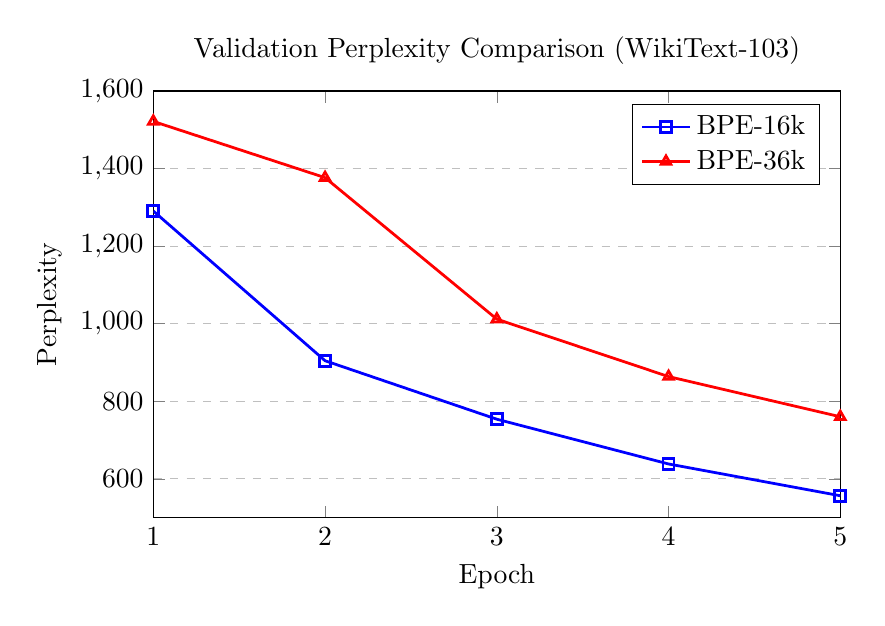
\begin{tikzpicture}
    \begin{axis}[
        title={Validation Perplexity Comparison (WikiText-103)},
        xlabel={Epoch},
        ylabel={Perplexity},
        xmin=1, xmax=5,
        ymin=500, ymax=1600,
        xtick={1,2,3,4,5},
        ytick={600, 800, 1000, 1200, 1400, 1600},
        legend pos=north east,
        ymajorgrids=true,
        grid style=dashed,
        width=0.85\textwidth,
        height=7cm,
    ]

    % K=16,000 Trend
    \addplot[
        color=blue,
        mark=square,
        line width=1pt,
        ]
        coordinates {
        (1, 1290.46)(2, 904.46)(3, 753.66)(4, 638.25)(5, 556.34)
        };
        \addlegendentry{BPE-16k}

    % K=36,000 Trend
    \addplot[
        color=red,
        mark=triangle,
        line width=1pt,
        ]
        coordinates {
        (1, 1521.50)(2, 1376.46)(3, 1011.68)(4, 863.56)(5, 759.99)
        };
        \addlegendentry{BPE-36k}

    \end{axis}
    \end{tikzpicture}
    \caption{Evolution of Validation Perplexity over 5 epochs for different vocabulary sizes.}
    \label{fig:ppl_k_comparison}
\end{figure}

The comparison between different vocabulary budgets on the WikiText-103 dataset reveals an interesting counter-intuitive result:
\begin{itemize}
    \item \textbf{Convergence Rate:} Contrary to the expectation that a larger vocabulary ($K=36k$) would facilitate better learning, the $K=16k$ configuration achieved a significantly lower final validation perplexity. This suggests that for a model of this scale (LSTM with 256 hidden units), a smaller, more dense vocabulary allows the model to learn token representations more effectively, as the parameter space for the embedding layer is smaller and easier to optimize.
    \item \textbf{Training Throughput:} There is a notable difference in computational cost. The $K=16k$ model trained significantly faster than the $K=36k$ model. This overhead is due to the larger Softmax layer at the output, which must compute probabilities over a wider range of tokens.
    \item \textbf{Information Bottleneck:} The higher perplexity of BPE-36k indicates that with a limited hidden size, increasing $K$ too much may lead to "sparsity" in token occurrences during training. The $K=16k$ model benefits from seeing each subword unit more frequently.
\end{itemize}

\subsubsection{Analysis of Tokenizers Impact on Language Model Performance}
To further examine the trade-offs across all tokenization families, we focus on five representative Enwik8 runs to compare perplexity and training speed under a fixed 3-epoch budget.

\begin{table}[H]
\centering
\caption{Enwik8 LM Results by Tokenizer Run (3 Epochs)}
\renewcommand{\arraystretch}{1.1}
\begin{tabular}{|l|c|c|c|}
\hline
\textbf{Tokenizer Run} & \textbf{Effective Vocab} & \textbf{Final Validation PPL} & \textbf{Avg Epoch Time (s)} \\ \hline
word\_2000 & 2000 & 20.853 & 107.805 \\ \hline
word\_36000 & 36000 & 91.595 & 247.414 \\ \hline
bpe\_2000 & 2000 & 53.018 & 540.036 \\ \hline
bpe\_36000 & 36000 & 178.612 & 255.976 \\ \hline
char\_2000 & 52 & 3.786 & 345.279 \\ \hline
\end{tabular}
\end{table}

\textbf{Perplexity and Speed Analysis:}
\begin{itemize}
    \item \textbf{Best Perplexity:} The character-level model obtains the lowest validation perplexity (3.786). However, this is achieved at a significant computational cost (345 s/epoch) due to sequence length.
    \item \textbf{Best Speed:} \texttt{word\_2000} is the fastest (107 s/epoch). Increasing the word vocabulary to 36k degrades both speed and perplexity, likely due to optimization sparsity.
    \item \textbf{BPE Scalability:} In BPE, increasing the vocabulary from 2k to 36k significantly improves speed (540s $\rightarrow$ 255s) because it shortens the sequences, though perplexity increases slightly under this fixed-epoch budget.
\end{itemize}

Under this specific configuration, \texttt{word\_2000} provides a strong speed-quality trade-off, while \texttt{char\_2000} minimizes perplexity at the cost of training time. BPE remains the most scalable solution for larger budgets and open-vocabulary scenarios.
